\documentclass[main.tex]{subfiles}

%\externalcitedocument{bibfile}

\begin{document}

Following the signal-like results from the 8-year analysis searching for matter enhanced oscillations with steriles, there was motivation to further explore the 3+1 phase space using multiple event morphologies. 
We first found that in the case of non-zero $\abs{U_{\mu 4}}^{2}$ and $\abs{U_{\tau 4}}^{2}$, a strong $\nu_{\tau}$ appearance signature could be expected; this is shown in Figure~\ref{fig:tau_oscillatiosn}.
Work was then carried out to predict IceCube's sensitivity to these $\nu_{\mu}\to\nu_{s}\to\nu_{\tau}$ oscillations using a joint track+cascade analysis and IceCube's latest public effective areas.
This work, published in Reference~\cite{PhysRevD.105.052001}, is included below.

\begin{figure}
    \centering
    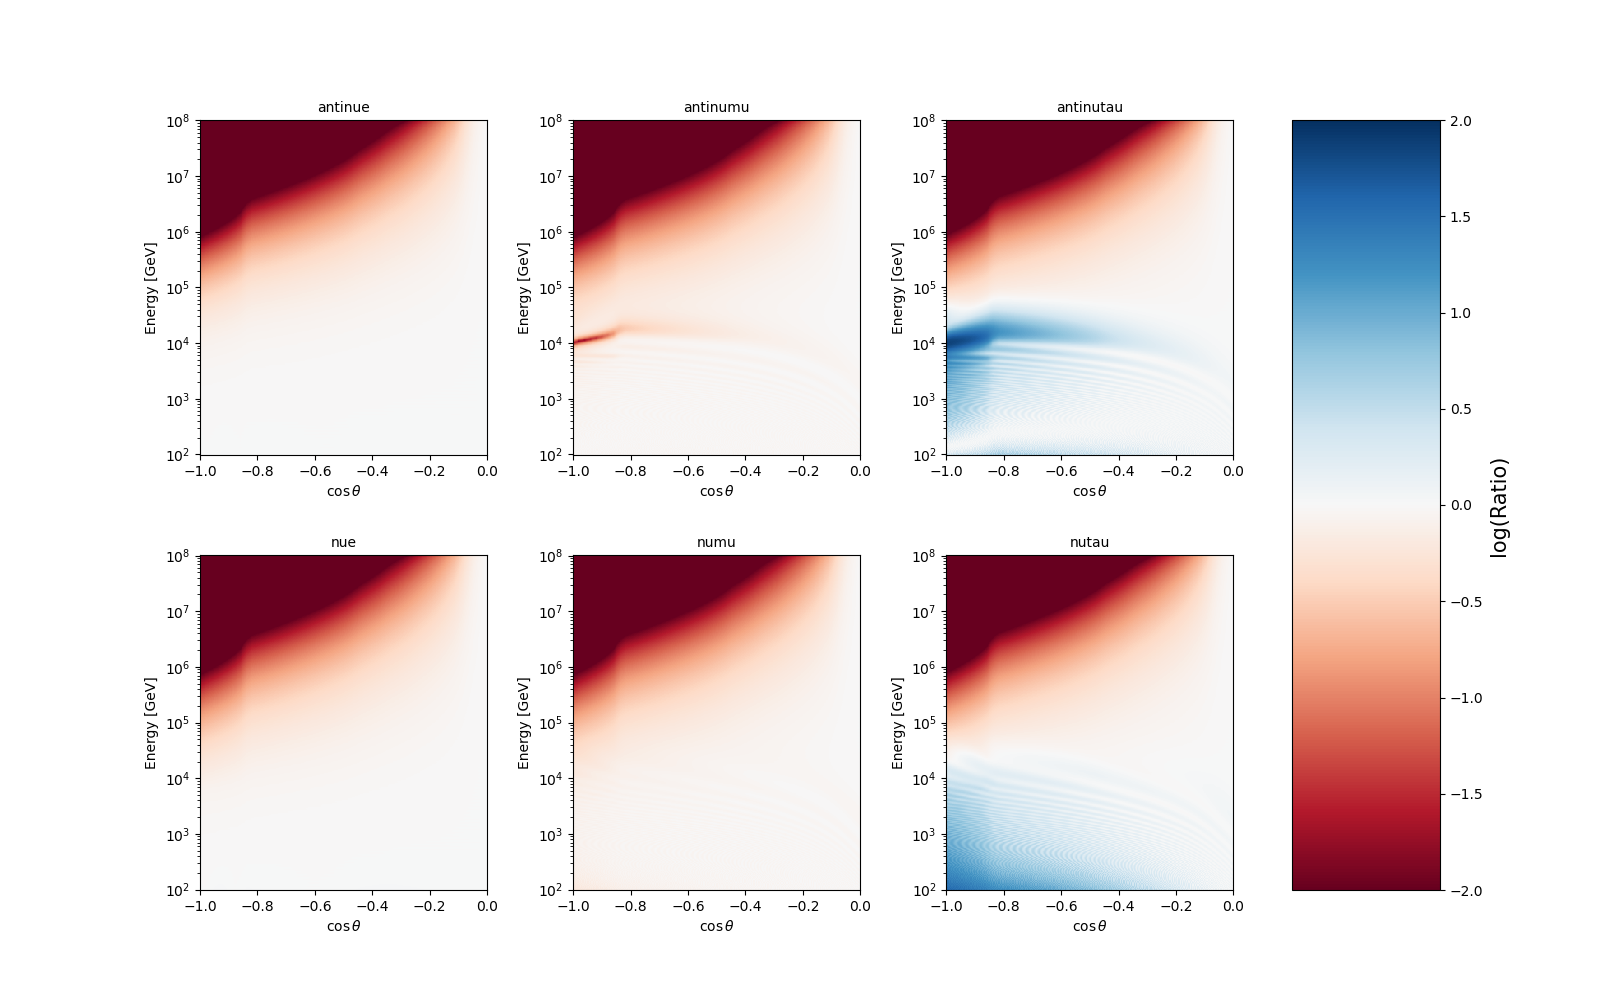
\includegraphics[width=0.8\linewidth]{figures/flux_plot_tau_appear.png}
    \caption{A plot showing the log of the ratio of the neutrino fluxes at the Earth's surface and the flux at IceCube. Like in Figure~\ref{fig:sterile_osc_sig}, the top let corner shows disappearance due to Earth's opacity to neutrinos at high energies and the narrow red band shows the MSW resonance with sterile neutrinos. Here, however, the blue region is showing an MSW-enhanced tau appearance signature for 3+1 sterile neutrino models with non-zero $\abs{U_{\tau4}}^{2}$.}\label{fig:tau_oscillatiosn}
\end{figure}

\includepdf[pages=-]{./cascades_sensitivity.pdf}

\end{document}